\documentclass[11pt,a4paper]{article}
\usepackage[T1]{fontenc}
\usepackage[utf8]{inputenc}
\usepackage[french]{babel}
\usepackage{lmodern,microtype,geometry,graphicx,booktabs,amsmath,float,caption}
\usepackage[hidelinks]{hyperref}
\geometry{margin=2.3cm}
\graphicspath{{../results/figures/}}
\newcommand{\tab}[1]{\resizebox{\linewidth}{!}{\input{tables/#1.tex}}}

\title{Maintenance prédictive par l'audio :\\ détection non supervisée de pannes de machines industrielles}
\author{Mohamed Aziz Ben Rejeb, Wael Znagui, Maram Nuigues,\\ Khalil Znazen, Aymen Turki\\[2pt] Mini-projet Deep Learning -- IIA5 -- INSAT\\ Encadrant : Ridha ALOUI}
\date{Décembre 2026}

\begin{document}
\maketitle

\begin{abstract}
Nous détectons des sons anormaux de pompes et de ventilateurs en n'apprenant que sur des sons normaux.
Trois approches sont comparées : un autoencodeur dense, un autoencodeur convolutif et des embeddings audio
pré-entraînés (PANNs) suivis d'un kNN ou d'un GMM. Sur DCASE 2020, notre autoencodeur dense retrouve la
baseline officielle (AUC 73,1 \% pour la pompe, 66,5 \% pour le ventilateur). Les embeddings avec un GMM par
machine donnent l'AUC la plus élevée sur la pompe (76,6 \%), mais aucune approche ne fait mieux que
l'autoencodeur dense sur le ventilateur. Sur un sous-ensemble de MIMII, les meilleures AUC passent d'environ
67--75 \% à $-6$~dB à environ 94 \% à $+6$~dB : le bruit est un facteur limitant majeur. Avec un seuil fixé sans aucune panne,
seules 41 \% (pompe) et 28 \% (ventilateur) des pannes sont détectées par l'autoencodeur dense, pour 11 à 14 \% de fausses alertes.
\end{abstract}

\section{Problématique}
Une machine qui se dégrade change souvent de son avant de tomber en panne. Les pannes étant rares et variées,
il est peu réaliste d'en collecter assez pour entraîner un classifieur. La question est donc : \emph{peut-on détecter
les anomalies à partir d'enregistrements audio, en n'apprenant que sur des sons normaux, et de façon robuste au bruit
d'usine ?} Le modèle produit un score d'anomalie par extrait ; un seuil transforme ce score en alerte.

\section{Données}
\paragraph{DCASE 2020 Task 2 (jeu de développement)~\cite{zenodo,koizumi}.} Extraits d'environ 10~s à 16~kHz, issus de
MIMII~\cite{purohit} pour les deux types retenus, pompe et ventilateur, avec 4 machines (ID 00, 02, 04, 06) par type.
L'entraînement ne contient que des sons normaux (3349 extraits pour la pompe, 3675 pour le ventilateur). Le test contient
400 normaux et 456 anormaux (pompe), 400 normaux et 1475 anormaux (ventilateur). Nous mettons de côté 10 \%
des normaux d'entraînement de chaque machine (validation), utilisés uniquement pour fixer les seuils.

\paragraph{MIMII, étude du bruit~\cite{purohit}.} Trois rapports signal sur bruit (RSB) : $-6$, 0 et $+6$~dB. Le jeu complet pesant
plusieurs dizaines de Go, nous utilisons un sous-ensemble fixe : par machine, 200 normaux (135 entraînement, 15 validation,
50 test) et 50 anormaux (test), un seul microphone, et les mêmes fichiers et le même découpage à chaque RSB. Les modèles
DCASE ne sont jamais testés sur MIMII, car DCASE en est dérivé (risque de fuite de données).

\section{Méthode}
\paragraph{Prétraitement.} Log-mel spectrogramme : 128 bandes, fenêtre de 1024 points, saut de 512, soit 313 trames pour 10~s.

\paragraph{Autoencodeur dense.} Architecture de la baseline officielle~\cite{koizumi} : vecteurs de 5 trames ($5\times128=640$),
couches 640--128$\times$4--8--128$\times$4--640 ; 100 époques, Adam ($10^{-3}$), lots de 512, un modèle par type de machine.
Le score est l'erreur quadratique moyenne de reconstruction.

\paragraph{Autoencodeur convolutif.} Patchs de $128\times64$ standardisés par bande mel, quatre convolutions à pas 2,
goulot de dimension 40, décodeur symétrique ; 80 époques, politique OneCycle ($2\cdot10^{-3}$).

\paragraph{Embeddings PANNs~\cite{kong}.} CNN14 pré-entraîné sur AudioSet, non réentraîné : un vecteur de 2048 valeurs par extrait,
standardisé. Deux scores : distance cosinus moyenne aux 5 plus proches voisins normaux (kNN), ou log-vraisemblance négative d'un
GMM à 2 composantes après ACP (32 dimensions). Deux portées : un détecteur \emph{par type}, comme les
autoencodeurs, ou \emph{par ID}, ce qui suppose de savoir quelle machine est écoutée.

\paragraph{Protocole.} Les hyperparamètres ci-dessus ont été fixés a priori ; aucun n'a été réglé sur les anomalies de test et toutes les
variantes sont rapportées. Le seuil est le 90\textsuperscript{e} ou 95\textsuperscript{e} percentile des scores de validation, par machine.
Les métriques sont l'AUC et la pAUC ($p=0{,}1$), moyennées sur les 4 machines. Les intervalles à 95 \% viennent d'un
bootstrap des extraits de test (1000 tirages) : ils ne mesurent pas la variabilité due à l'entraînement, effectué une seule fois.

\paragraph{Calcul et contrôle des entraînements.} Les entraînements ont été faits sur GPU Tesla T4 (Kaggle). Une première tentative sur un
GPU portable (GTX 1650) a produit des gradients faux par intermittence (de l'ordre de $10^{7}$ à $10^{8}$, contre 0,1 en rejouant le même calcul sur CPU) ;
ces résultats ont été écartés. La cause probable, non démontrée, est la surchauffe (92--93~$^\circ$C). Un contrôle arrête désormais
un entraînement dont le gradient maximal dépasse $10^4$ fois la médiane, ou dont la perte augmente de plus de 50 \% d'une époque à l'autre. Une première limite de 100 avait arrêté
à tort deux entraînements sains ; elle a été relevée au vu des gradients et des pertes, pas des scores de test.

\section{Résultats sur DCASE}
\begin{figure}[H]\centering
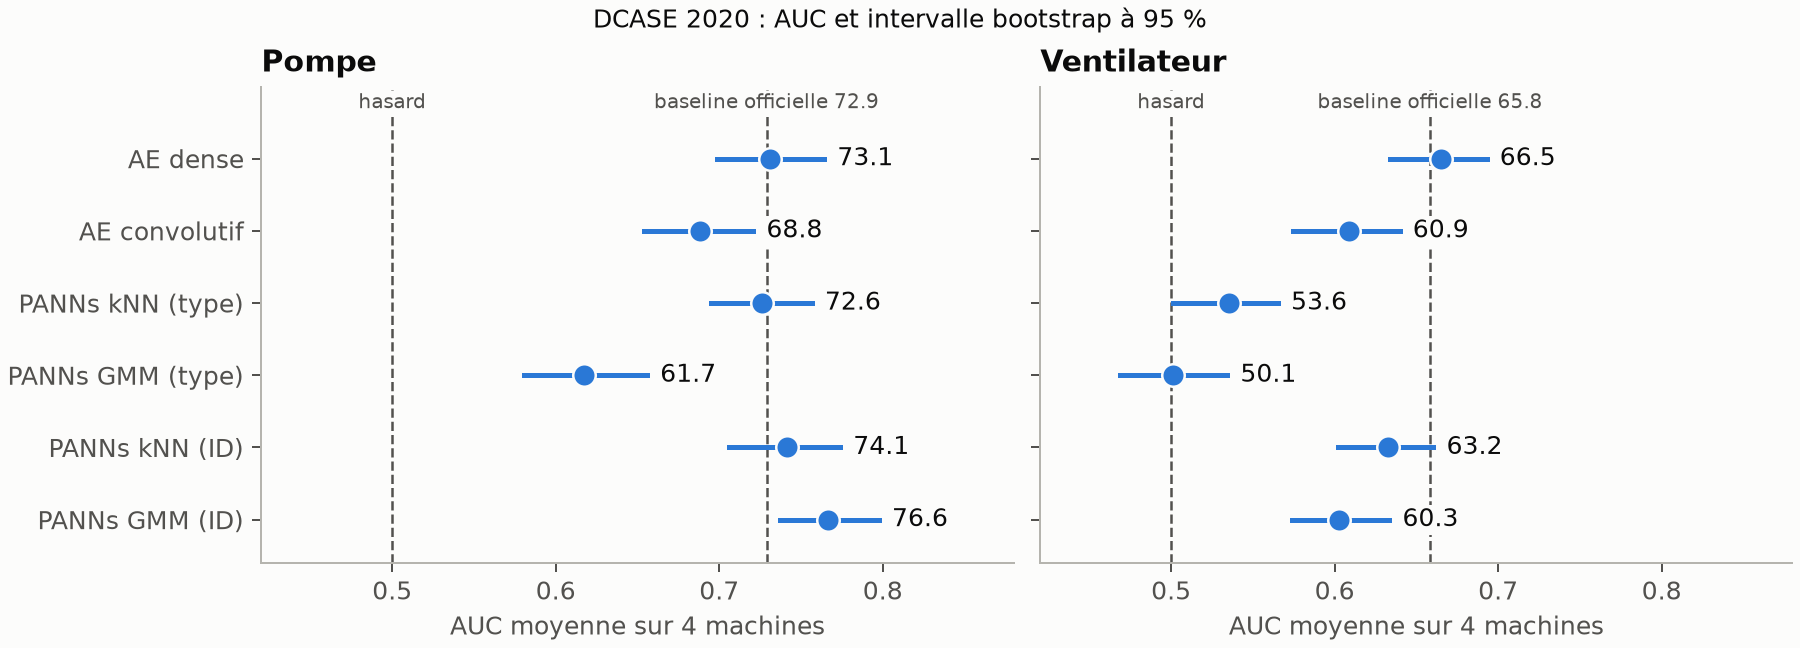
\includegraphics[width=.95\linewidth]{dcase_auc.png}
\caption{AUC moyenne et intervalle à 95 \%. Baseline officielle : moyenne de 10 entraînements~\cite{koizumi}.}
\end{figure}

\begin{table}[H]\centering
\caption{DCASE : AUC / pAUC (\%) par machine et par modèle. Baseline officielle : 72,89 / 59,99 (pompe) et 65,83 / 52,45 (ventilateur).}
\label{tab:dcase}
\tab{dcase}
\end{table}

\begin{itemize}
\item \textbf{L'autoencodeur dense reproduit la baseline}, ce qui valide notre chaîne de traitement.
\item \textbf{L'autoencodeur convolutif est moins bon que le dense} en moyenne, de 4 à 6 points. Il obtient 93,3 \% sur la pompe id\_04, mais 48,8 \%
(le hasard) sur id\_02. Une explication possible est qu'il reconstruit trop bien certaines anomalies ; nous ne l'avons pas vérifiée.
\item \textbf{PANNs : intéressant pour la pompe, faible pour le ventilateur.} Le GMM par ID atteint 76,6 \% sur la pompe, avec un intervalle (73,7--79,8)
qui recouvre celui du dense (69,9--76,4). À portée égale (par type), aucune variante PANNs ne dépasse l'autoencodeur dense.
\item \textbf{Les résultats varient beaucoup selon la machine.} Les ventilateurs id\_00 et id\_04 sont difficiles pour toutes les approches.
\item \textbf{La pAUC reste faible} (51 à 62 \% en moyenne) : peu de pannes sont détectables à bas taux de fausses alertes.
\end{itemize}
La meilleure variante PANNs est identifiée a posteriori sur le test : sa valeur est donc légèrement optimiste.

\section{Seuil d'alerte}
\begin{table}[H]\centering
\caption{DCASE : décision (\%), 4 machines regroupées. « Alerte permanente » : alerte sur chaque extrait.}
\tab{decision}
\end{table}

\begin{figure}[H]\centering
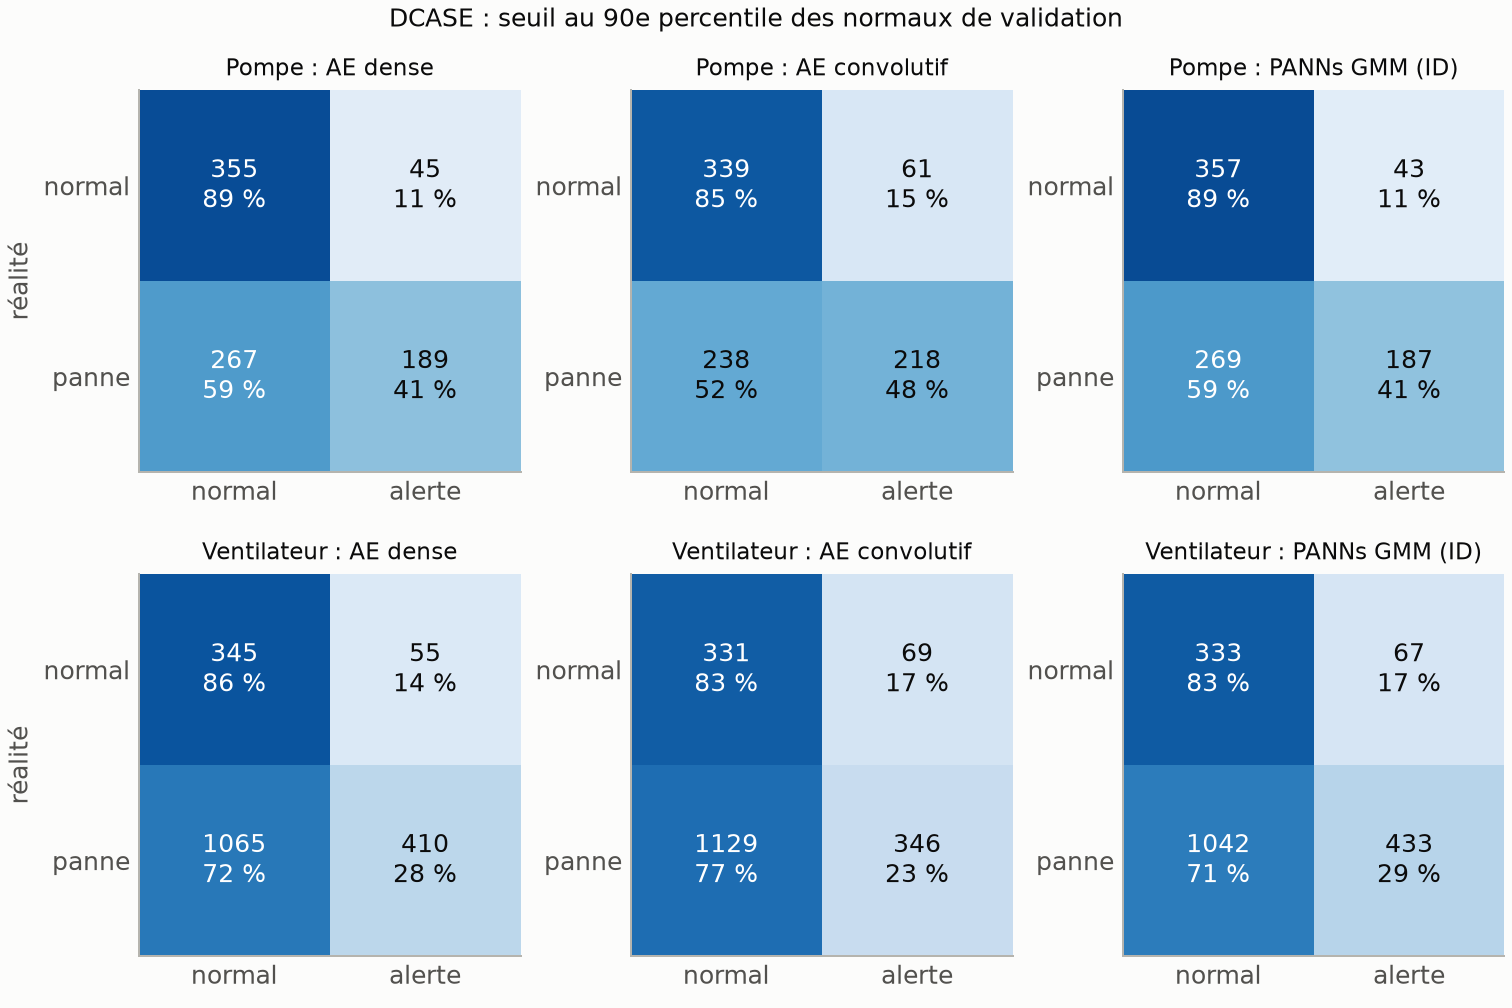
\includegraphics[width=.75\linewidth]{confusion_dcase.png}
\caption{Matrices de confusion au 90\textsuperscript{e} percentile.}
\end{figure}

Au 90\textsuperscript{e} percentile, l'autoencodeur dense détecte 41 \% des pannes de pompe (11 \% de fausses alertes) et 28 \% de celles du
ventilateur (14 \%). La majorité des pannes est donc manquée. Le taux visé de 10 \% de fausses alertes est généralement dépassé :
le seuil se transfère imparfaitement de la validation au test.

La précision et le F1 doivent être lus avec prudence : le test DCASE contient 53 \% (pompe) et 79 \% (ventilateur) d'anomalies, et une alerte permanente, inutile
en pratique, aurait un F1 supérieur à celui de tous nos modèles. L'exactitude équilibrée est plus informative. Dans une
usine où les pannes sont rares, la précision serait bien plus basse.

\section{Robustesse au bruit}
\begin{figure}[H]\centering
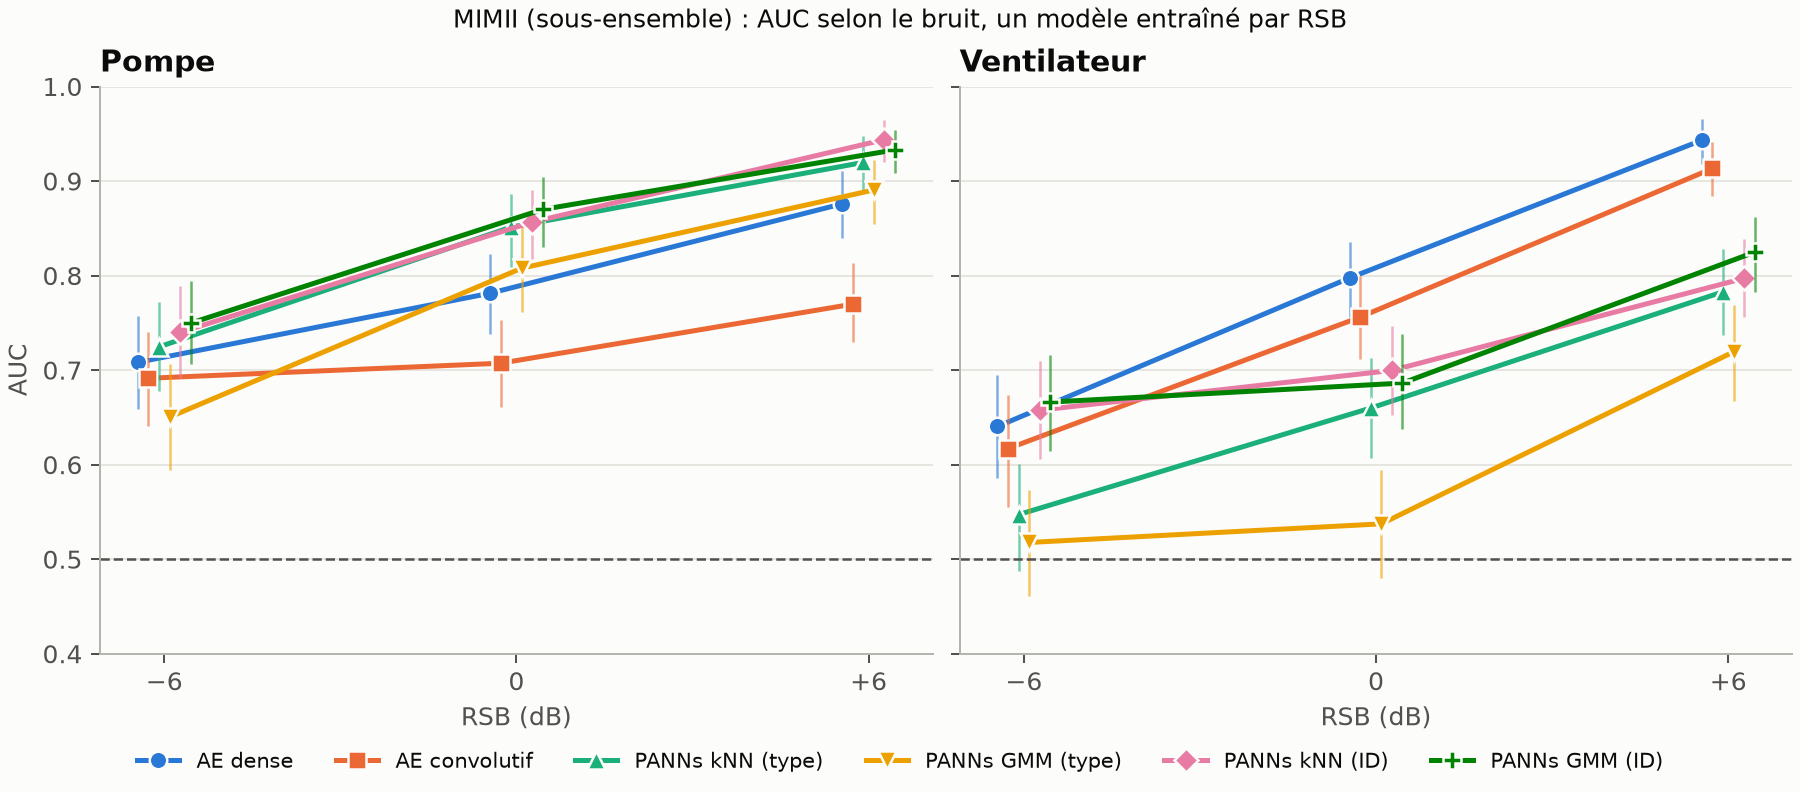
\includegraphics[width=\linewidth]{noise_auc.png}
\caption{MIMII : AUC selon le RSB, avec intervalles à 95 \%. Points décalés horizontalement pour la lisibilité.}
\end{figure}

\begin{table}[H]\centering
\caption{MIMII : AUC / pAUC (\%), moyenne des 4 machines.}
\begin{tabular}{llccc}
\toprule
Machine & Modèle & -6 dB & 0 dB & +6 dB \\
\midrule
Pompe & AE dense & 70,8 / 59,9 & 78,1 / 65,4 & 87,6 / 85,3 \\
Pompe & AE conv. & 69,1 / 61,7 & 70,7 / 65,3 & 77,0 / 80,9 \\
Pompe & kNN type & 72,5 / 59,2 & 85,1 / 68,7 & 92,0 / 74,4 \\
Pompe & GMM type & 65,0 / 56,7 & 80,8 / 64,3 & 89,1 / 72,3 \\
Pompe & kNN ID & 74,0 / 56,4 & 85,7 / 68,5 & 94,4 / 81,9 \\
Pompe & GMM ID & 75,0 / 56,7 & 87,0 / 75,7 & 93,3 / 79,5 \\
\midrule
Ventilateur & AE dense & 64,0 / 52,3 & 79,8 / 62,6 & 94,3 / 81,6 \\
Ventilateur & AE conv. & 61,7 / 52,9 & 75,6 / 60,7 & 91,3 / 78,2 \\
Ventilateur & kNN type & 54,7 / 52,7 & 66,0 / 52,1 & 78,3 / 58,9 \\
Ventilateur & GMM type & 51,8 / 51,5 & 53,7 / 50,3 & 71,9 / 53,8 \\
Ventilateur & kNN ID & 65,8 / 53,9 & 70,0 / 58,6 & 79,7 / 65,9 \\
Ventilateur & GMM ID & 66,6 / 53,8 & 68,6 / 57,8 & 82,5 / 65,3 \\
\bottomrule
\end{tabular}
\end{table}

Toutes les approches progressent quand le bruit diminue, de 8 à 30 points d'AUC entre $-6$ et $+6$~dB. La meilleure approche dépend de la machine :
PANNs pour la pompe, l'autoencodeur dense pour le ventilateur à 0 et $+6$~dB. Le ventilateur n'est donc pas intrinsèquement
indétectable : l'autoencodeur dense y atteint 94,3 \% à $+6$~dB. À $-6$~dB, les écarts entre les meilleures approches sont dans
la marge d'incertitude. Il n'y a que 100 extraits de test par machine, et le modèle est réentraîné à chaque RSB :
un changement de bruit après déploiement, non testé ici, serait sans doute plus pénalisant.

\section{Cartes d'erreur}
\begin{figure}[H]\centering
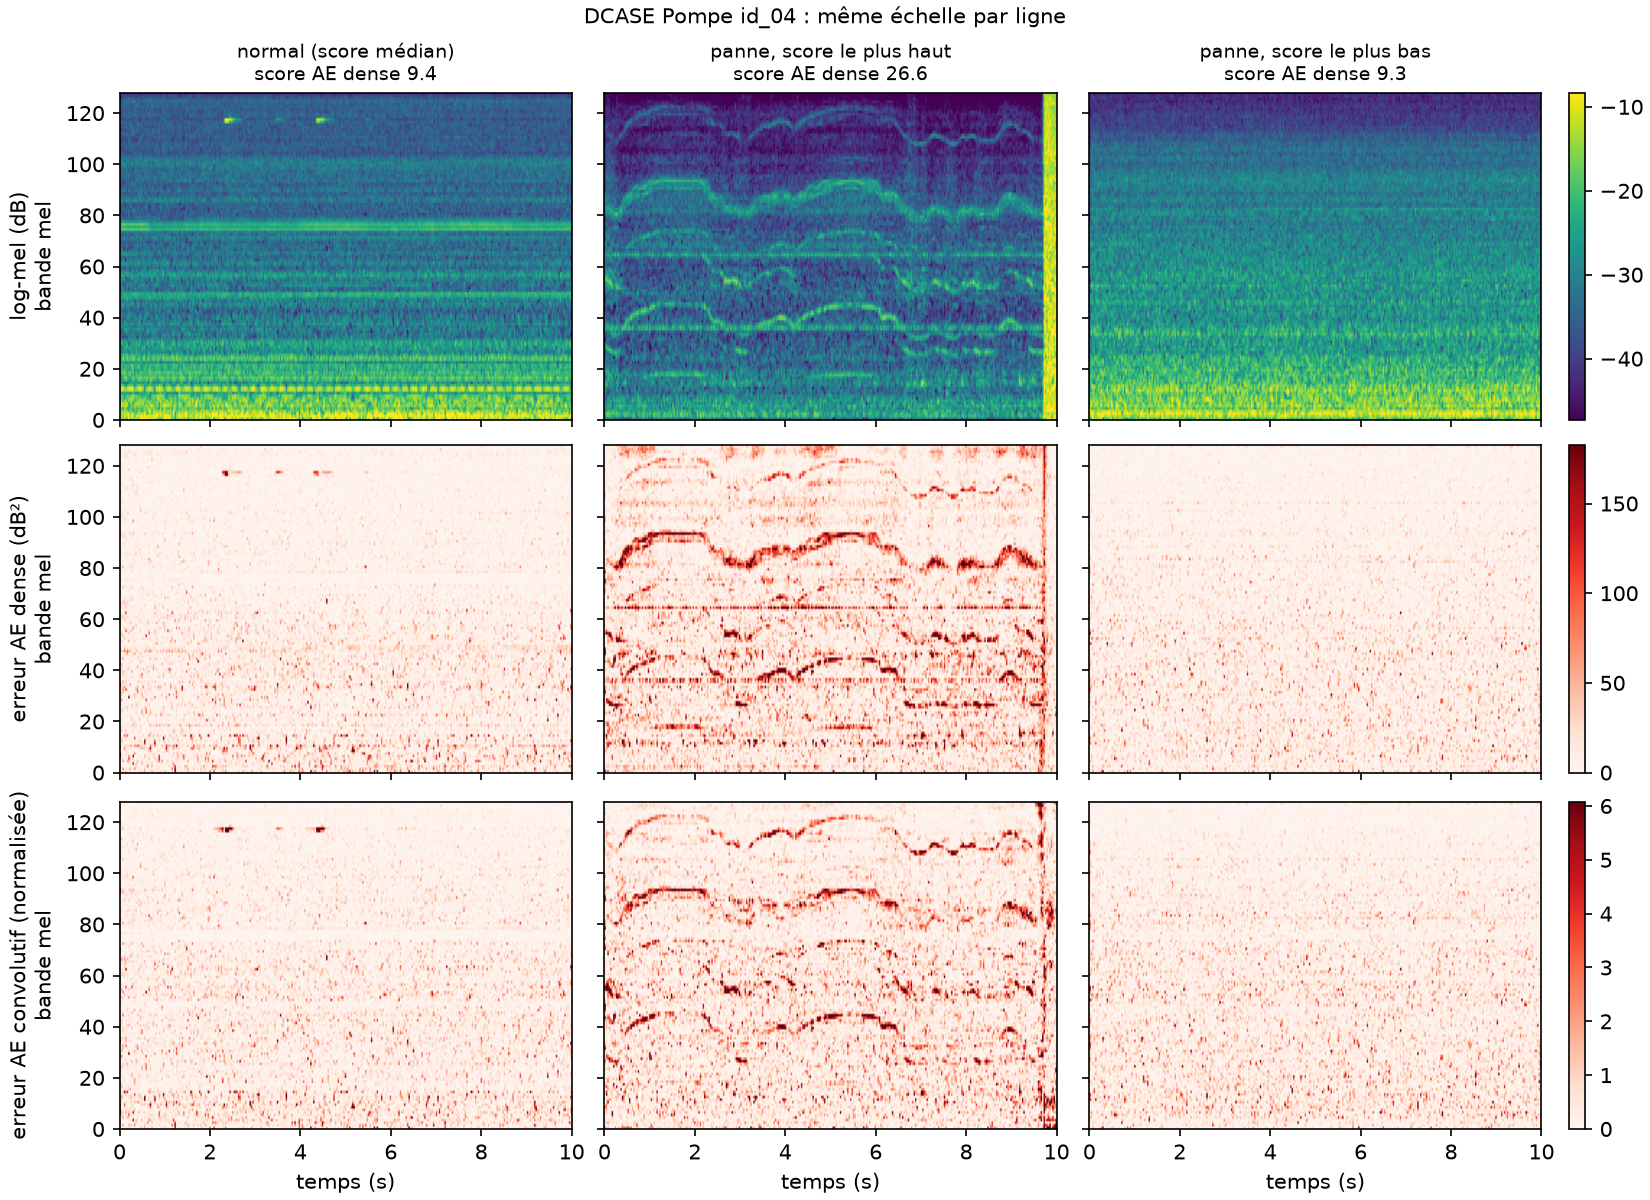
\includegraphics[width=.86\linewidth]{error_map_pump.png}
\caption{Pompe id\_04 : spectrogrammes et erreurs de reconstruction.}
\end{figure}
\begin{figure}[H]\centering
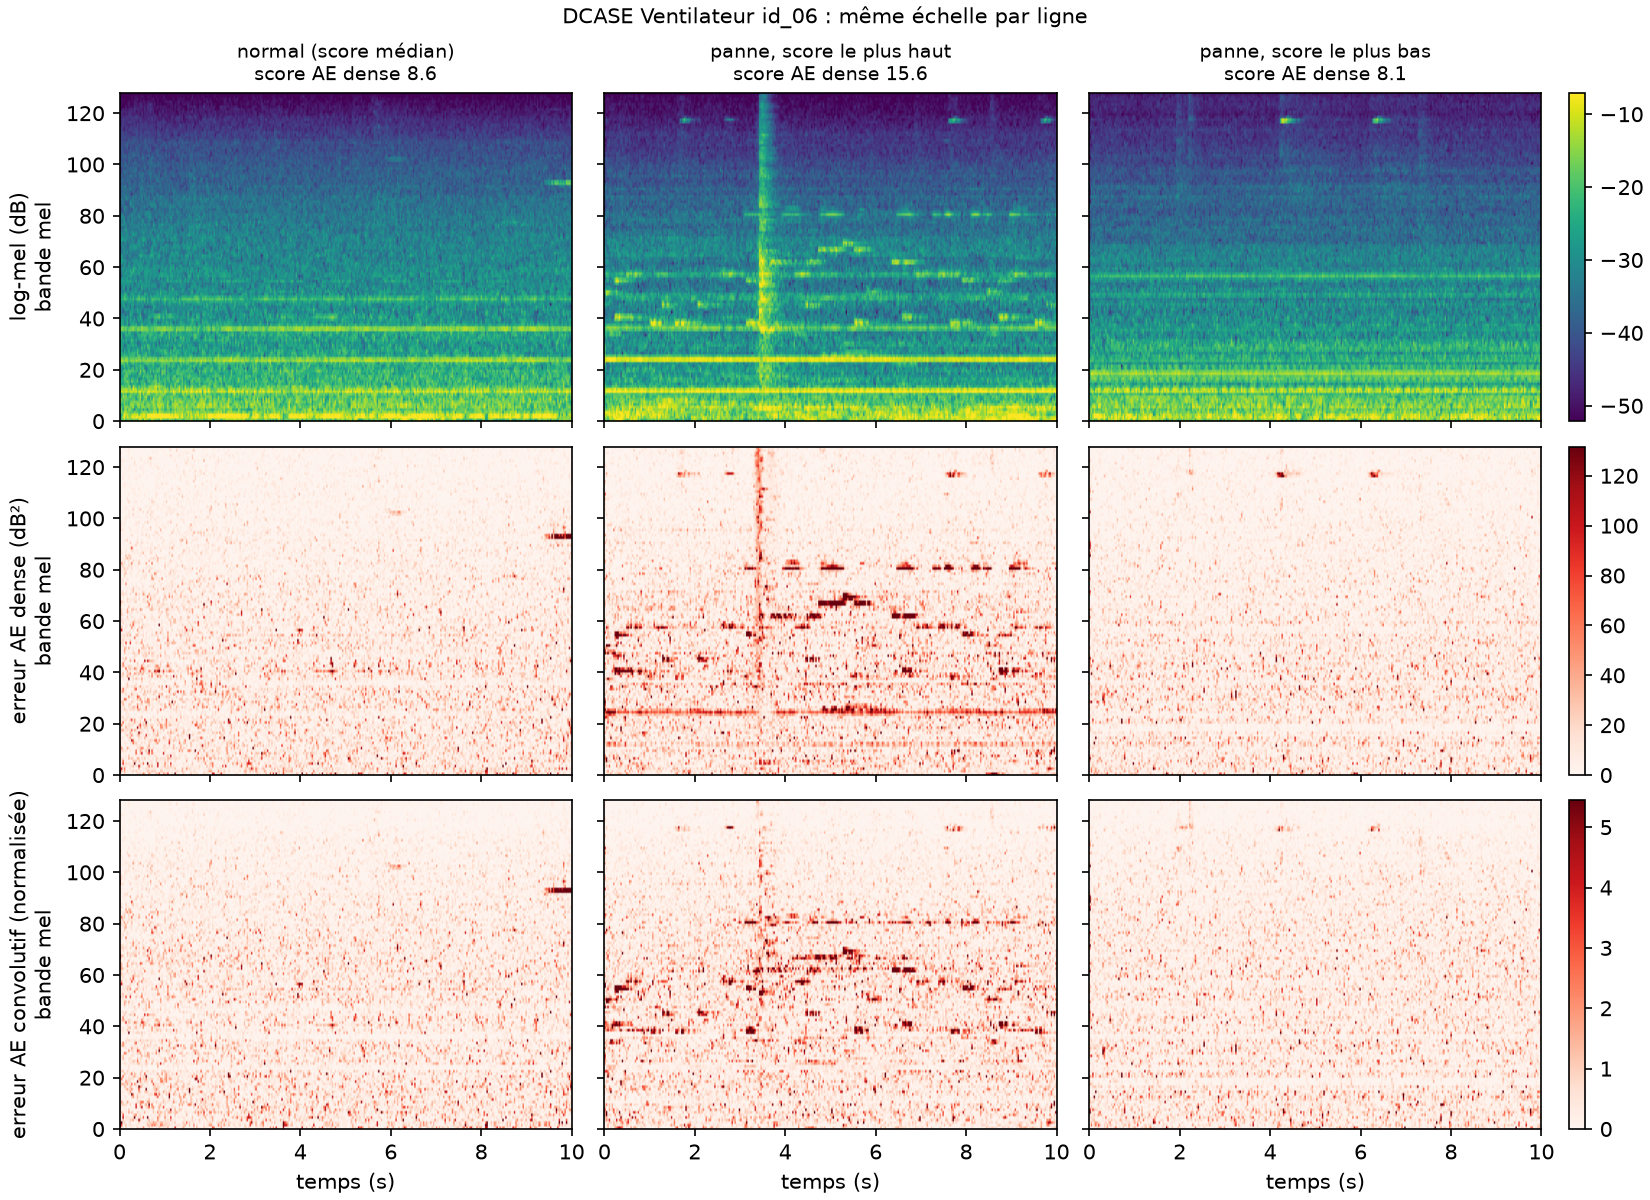
\includegraphics[width=.86\linewidth]{error_map_fan.png}
\caption{Ventilateur id\_06 : spectrogrammes et erreurs de reconstruction.}
\end{figure}
Les extraits sont choisis par règle : pour la machine de meilleure AUC dense, le normal de score médian et les pannes de score le plus haut et le plus bas.
Les cartes localisent l'anomalie en temps et en fréquence : sur la pompe, l'erreur suit les raies mobiles. La panne de score le plus bas
ressemble à un son normal pour le modèle. Sur le ventilateur, l'erreur vient de notes brèves et d'un choc qui pourraient
être du bruit d'usine : \textbf{un score élevé signale un son inhabituel, pas nécessairement une panne}.

\section{Déploiement : ONNX, INT8 et latence CPU}
\begin{table}[H]\centering
\caption{Taille, AUC (\%) et latence du modèle par extrait de 10~s (médiane de 200 mesures, 1 thread, Intel i5-10300H).}
\begin{tabular}{llcccc}
\toprule
Modèle & Version & Taille (Ko) & AUC pompe & AUC vent. & Latence (ms) \\
\midrule
AE dense & FP32 & 1061 & 73,1 & 66,5 & 2,5 \\
AE dense & INT8 statique & 325 & 73,7 & 63,8 & 2,8 \\
AE dense & INT8 dynamique & 299 & 73,0 & 66,7 & 3,0 \\
AE conv. & FP32 & 1490 & 68,8 & 60,9 & 11,7 \\
AE conv. & INT8 statique & 430 & 70,1 & 59,2 & 8,0 \\
\bottomrule
\end{tabular}
\end{table}
La lecture de l'audio et le log-mel ajoutent 5,0~ms. La calibration statique utilise 100 sons normaux d'entraînement. Pour l'autoencodeur dense, l'INT8 dynamique divise la taille par 3,5 sans
perte notable d'AUC ; l'INT8 statique perd 2,7 points sur le ventilateur. Les gains apparents sur la pompe sont des effets d'arrondi. L'INT8 n'accélère pas le dense, déjà très petit, mais réduit la
latence du convolutif d'environ 30 \%. CNN14 demande 820~ms sous PyTorch et 80 millions de paramètres : environ 100 fois plus lent que la
chaîne dense complète, pour 3,5 points d'AUC sur la pompe. Les scores changent après quantification : les seuils doivent être recalculés.
Ces mesures viennent d'un ordinateur portable, pas d'une carte embarquée.

\section{Démonstrateur}
Une application Gradio (CPU, ONNX) accepte un fichier ou un enregistrement au microphone et affiche le score, le verdict, le spectrogramme
et la carte d'erreur. Les exemples fournis sont des extraits de score médian ; la panne de ventilateur y est manquée, ce qui illustre
les limites mesurées. Les seuils ne valent que pour ces machines et ces conditions d'enregistrement.

\section{Limites}
\begin{itemize}
\item Deux types de machines seulement, et un sous-ensemble réduit de MIMII (15 sons de validation par machine).
\item Un seul entraînement par modèle : la variabilité due à l'initialisation n'est pas mesurée.
\item Les détecteurs par ID disposent d'une information que les autoencodeurs par type n'ont pas.
\item Score moyen par extrait : une anomalie brève peut être diluée.
\item Pas d'essai sur une autre usine, un autre microphone ou une vraie carte embarquée.
\end{itemize}

\section{Conclusion}
Il est possible de détecter des anomalies en n'apprenant que sur des sons normaux, mais la fiabilité dépend fortement de la machine et du bruit.
Un modèle plus complexe n'est pas toujours meilleur : l'autoencodeur dense, très léger, est difficile à battre sur le ventilateur, tandis que les embeddings
pré-entraînés apportent un gain sur la pompe pour un coût de calcul bien plus élevé. En l'état, le système peut aider un technicien à
repérer des sons inhabituels, mais il manque trop de pannes pour remplacer une surveillance. Pistes : autoencodeurs par machine,
score sur les trames les plus anormales, apprentissage auto-supervisé utilisant l'ID, seuils recalibrés sur site.

\begin{thebibliography}{9}
\bibitem{zenodo} Y.~Koizumi et al., \emph{DCASE 2020 Challenge Task 2 Development Dataset}, Zenodo, 2020. \url{https://zenodo.org/records/3678171}. Licence CC BY-NC-SA 4.0.
\bibitem{purohit} H.~Purohit et al., « MIMII Dataset: Sound Dataset for Malfunctioning Industrial Machine Investigation and Inspection », \emph{DCASE Workshop}, 2019. \url{https://zenodo.org/records/3384388}. Licence CC BY-SA 4.0.
\bibitem{koizumi} Y.~Koizumi et al., « Description and Discussion on DCASE2020 Challenge Task2: Unsupervised Anomalous Sound Detection for Machine Condition Monitoring », \emph{DCASE Workshop}, 2020.
\bibitem{kong} Q.~Kong et al., « PANNs: Large-Scale Pretrained Audio Neural Networks for Audio Pattern Recognition », \emph{IEEE/ACM Transactions on Audio, Speech, and Language Processing}, vol.~28, 2020. Poids : \url{https://zenodo.org/records/3987831}.
\end{thebibliography}
\end{document}
